\documentclass[journal]{IEEEtran}
\ifCLASSINFOpdf
\else
\fi
\hyphenation{}
\usepackage{amsmath,amssymb,amsthm}
\usepackage{xparse}
\usepackage{latexsym}
\usepackage{amsfonts}
\usepackage{graphicx}
\usepackage{txfonts}
\usepackage{wasysym}
\usepackage{enumitem}
\usepackage{adjustbox}
\usepackage{ragged2e}
\usepackage{tabularx}
\usepackage{changepage}
\usepackage{setspace}
\usepackage{hhline}
\usepackage{multicol}
\usepackage{float}
\usepackage{multirow}
\usepackage{makecell}
\usepackage{fancyhdr}
\usepackage[toc,page]{appendix}
\usepackage[utf8]{inputenc}
\usepackage[T1]{fontenc}
\usepackage{hyperref}
\usepackage{isomath}
\usepackage{fixmath}
\usepackage{tikz}
\usepackage{textcomp}
\usepackage{epstopdf} %converting to PDF
\usepackage{upgreek}
\usepackage{mathtools}
\usepackage{xfrac}
\usepackage{lipsum}
\usepackage[colorinlistoftodos]{todonotes}
\input{./Modules/LatexShortcuts_Itayyeka_2.tex}
%%%%%%%%%%%%%%    aliases    %%%%%%%%%%%%%%
\newcommand{\dTheta}{\Delta\theta}
\newcommand{\dTau}{\Delta\tau}
\newcommand{\D}[2]{\mathcal{D}\left(#1,#2\right)}
\newcommand{\Dp}[3]{\mathcal{D}^{#3}\left(#1,#2\right)}
\newcommand{\fbBpRatio}{
\left|
\frac{
\frac
{
\vecnot{\alpha}^{T}\vecnot{d}_{\theta_{s}}exp\left(-j\tau_{s}\right)
}
{
4c^{2}\tau_{s}^{2}-\vecnot{\beta}^{T}\vecnot{d}_{\theta_{s}}exp\left(-j\tau_{s}\right)
}
}{
\frac
{
\vecnot{\alpha}^{T}\vecnot{d}_{\theta}exp\left(-j\tau\right)
}
{
4c^{2}\tau^{2}-\vecnot{\beta}^{T}\vecnot{d}_{\theta}exp\left(-j\tau\right)
}
}
\right|
}
\newcommand{\Hr}[3]{\mathcal{H}^{#3}\left(#1,#2\right)}
\newcommand{\Steer}[1]{\vecnot{d}_{#1}}

\NewDocumentCommand{\evalat}{sO{\big}mm}{%
  \IfBooleanTF{#1}
   {\mleft. #3 \mright|_{#4}}
   {#3#2|_{#4}}%
}

\newcommand{\hDen}{\left(4c^{2}\tau^{2}-\vecnot{\beta}^{T}\vecnot{d}e^{-j\omega\tau}\right)}
%%%%%%%%%%%%%%%%%%%%%%%%%%%%%%%%%%%%%%%%%%%%%%%%%%%%%%
%%%%%%%%%%%%%%      Document flags     %%%%%%%%%%%%%%%
%%%%%%%%%%%%%%%%%%%%%%%%%%%%%%%%%%%%%%%%%%%%%%%%%%%%%%
% \def\showDev{}
\def\DEFIncludeAttenuation
%%%%%%%%%%%%  Document Code starts here %%%%%%%%%%%%%%
\begin{document}
\title{Source Localization With Feedback Based Beamforming}
\author{Itay Yehezkel Karo,~\IEEEmembership{}
        Tsvi G. Dvorkind~\IEEEmembership{}
        and 
        Israel Cohen,~\IEEEmembership{Fellow,~IEEE}
\thanks{Andrew and Erna Viterby Faculty of Electrical Engineering, Technion -- Israel Institute of Technology, Technion City, Haifa 3200003, Israel (e-mail: itayyeka@gmail.com, icohen@ee.technion.ac.il)}% <-this % stops a space
\thanks{T. G. Dvorkind is with Rafael corp.}% <-this % stops a space
}
\markboth{}%
{}
\maketitle
\begin{abstract}
State-of-the-art array processing methods, ranging from high-order statistics to adaptive configuration, demand costly computing effort in pursuit for spatial performance improvement.
% State-of-the-art sensor arrays use a variety of methods, ranging from high-order statistics to adaptive configuration, to improve spatial performance, all of which demand costly computing effort.
A feedback based approach is introduced in the context of localization, featuring low complexity and high spatial performance in the excess of integrating a transmitter to the array.  
In the proposed scheme, a signal is continuously re-transmitted between the array and the target of interest.
Considering ideal scenarios, the feedback based beamformer virtually achieves infinite aperture, increasing the available spatial information about the target and significantly improves the array's spatial performance.
Using traditional beamforming performance analysis, the beamwidth, peak to side-lobe ratio, array directivity and white noise sensitivity are evaluated considering the feedback based array.
Then, significant improvement in all aspects is shown, while thoroughly discussing the conditions for enhanced performance.
Finally, an application of low estimation errors sensitivity, featuring high performance even in low signal-to-noise ratio, is presented and analyzed, serving as a practical and robust implementation of the feedback based localization concept.
% Also, the suggested application features high performance in low signal-to-noise ratio.  
\end{abstract}
\begin{IEEEkeywords}
Spatial array processing, beamforming, source localization, beam-pattern, cooperative beamforming, spatial IIR.
\end{IEEEkeywords}
\section{Introduction}
\IEEEPARstart{T}{he} 
general field of array processing has been thoroughly studied in many contexts throughout several decades, producing many important application such as spatial filtering, source localization, signal detection, source separation, manifold learning, feature extraction, and many more.
Spatial sensor arrays enable the extraction of spatial information such as localizing a transmitting source \cite{skolnik2008radar} \myTodo{inline}{\textbf{DONE:}\\cite some radar book}, blindly separating mixtures of impinging signals \cite{Comon1994IndependentConcept} \myTodo{inline}{\textbf{DONE:}\\here you can cite some papers which talk about BSS and ICA signal source separation. Make sure to cite something which is well known, that is, has many citations}, improving signal to noise ratio (SNR) \myTodo{inline}{\textbf{DONE:}\\cite some works/books about MVDR,MPDR processing}\cite{Frost1972AProcessing,verdu1998multiuser} and many more. 
\par Uniform linear array (ULA), a uniformly spaced structure of sensors, has always been a point of interest, due to its simplicity of analysis \cite{VanTrees2002DetectionIV}. 
The array size and the number of its elements $N$ has significant influence on the obtained array performance, such as SNR improvement, spatial separation capabilities and its number of degrees of freedom (DOF). For example, the influential MUSIC algorithm \cite{Ralph1986MultipleParameter} enables to detect up to $N-1$ directions of arrival (DOA) due to $N-1$ spatially separated sources, by projecting the possible steering vectors (SV) of the array manifold onto the noise subspace.
The limitation on the number of processed or detected sources due to the limited amount of DOF of a given array, inspired different directions of research.\myTodo{inline}{\textbf{ACCEPTED:}\\you are focusing on the DOF problem, but this is not the main focus of our paper...} 
\par One approach, involving different array geometries, examined minimum redundancy arrays \cite{Moffet1968Minimum-RedundancyArrays,Pillai1985AEstimation,UnnikrishnaPillai1987StatisticalMatrix} \myTodo{inline}{are those the works were we look at arrays with 'holes' and fill in the void due to second order statistics across the existing elements?\\\textbf{ANSWER}\\ No, those works deal with non-uniform linear arrays, reducing the element spacing redundancy, such that for $N$ element array, there will be the minimal number of pair with a specific difference. The main purpose is to increase resolution by reducing ambiguity. The extraction of the "holes" is the "virtual array" concept which is mentioned next} trying to reduce the spatial ambiguity through minimization of redundant inter-element spacing in order to increase the overall resolution. 
\par Another approach, commonly referenced as ``virtual arrays" \cite{Pal2010NestedFreedom,Chevalier2005OnProcessing,Mendel1999ApplicationsProcessing}\myTodo{inline}{are you citing known works? \\\textbf{(Yes, for example \cite{Chevalier2005OnProcessing} is cited ~200 times)}\\ I think Veydanathan \\\textbf{ADDED his work.}\\(hope that spelling correctly) did some works on this. Also Arye Yeredor from TAU} deals with the extraction of samples originated in sensors that do not really exist (i.e. relying on higher order statistics and manipulating multiple statistical cross-terms in order to estimate statistical characteristics of signals impinging in missing sensors). 
Using a similar approach, the $2q$-MUSIC algorithm \cite{Chevalier2006High-resolutionAlgorithm} \myTodo{inline}{not familiar... \\\textbf{Has around ~140 citations}\\}, enables the use of $N^{2q}$ ``virtual elements'', by calculating the $q$'th order statistics. \myTodo{inline}{\textbf{REPHRASED: and reduced}\\did not understand this last sentence. You did not explain what are nested arrays.}
\par A well known \cite{VanVeenBeamforming:Filtering} equivalence, which inspired the current paper, is the analogy between ULA spatial array processing of narrow-band signals and finite impulse response (FIR) temporal filtering. 
In the context of temporal signal processing, it is well known that for a given filter order $N$, in many cases, the infinite impulse response (IIR) filter leads to improved performance, as compared to FIR filter design of the same order. In particular, narrow transition regions, and low sidelobes can be achieved by implementing feedback based filtering. 
\par This naturally arises the question, ``what are the equivalent spatial domain processing methods which will be analogous to temporal IIR filtering? " 
\par A related work \cite{Wen2013ExtendingStructure} has also addressed this question. 
There, in the context of ULA, two approaches were considered. \myTodo{inline}{\textbf{DONE:}\\The next sentence is not clear. Please rephrase}
The first one was to estimate the time of arrival (TOA) difference between two consecutive sensors and to synthetically generate the recursive part of the IIR filter, entirely in the time-domain. 
The second approach suggested to consider overlapping subsets of one large ULA as finite approximation to an infinite array. Surely, the former approach heavily relies on the accuracy of the delay estimation and the latter approach does not achieve a recursive spatial response. In both cases, there is no true spatial feedback between the array and the source of interest.
\par Other works \cite{Madanayake2008AFilters,Madanayake2008ABeamformer} use the concept of $2D$ spatio-temporal plane wave representation (i.e. a straight line angled according to the DOA in the spatio-temporal plane), to design ultra-wide-band (UWB) filters \cite{L.Bruton1983HighlyPlanes} which both sample spatial snapshots of the signal and recursively process it in temporal domain. \myTodo{inline} {\textbf{REPHRASED}\\please explain (maybe later just to me) how UWB filtering is used}\myTodo{inline}{\textbf{Removed - not important - a way of implementation}\\what is that?}\myTodo{inline}{\textbf{DONE:}\\what are the drawbacks if these last papers?}
Here as well, the recursive part of the filter is obtained entirely in the temporal domain.  
\par The goal in this contribution, is to present a sensor array processing approach which achieves spatial-domain feedback-based processing, similarly to IIR filtering in the time domain. Opposed the previous works, we do not wish to estimate the inter-element delay and apply the recursive part in the time domain, but rather implement the feedback entirely in the spatial domain.
We focus on a localization problem, where our goal is to estimate the direction and the range of some target.
Opposed to classical array processing, we incorporate spatial feedback, show its equivalence to IIR filtering in case of a ULA, and analyze some key aspects of the proposed scheme. 

The spatial feedback between the array and the target is created by constantly re-transmitting a signal and its echoes between the array and the target. 
The initial stimulus can be generated at the target itself or at the location of the array. In the text to follow, we assume this is the latter. 

Also, similar to radar applications, the target can be passive and merely reflect the impinging signal, or to be cooperative, i.e. by receiving, enhancing the signal and re-transmitting it back to the array. In this work, we assume the former.

\par The outline of this paper is as follows. We first formulate the classic spatial beamforming setup in Sec.~\ref{sec:setup}. Then, in Sec.~\ref{sec_introduceFeedback}, we propose our novel feedback based architecture, and calculate its spatial response. In Sec.~ \ref{sec_FIM} we evaluate the Fisher Information Matrix (FIM) and discuss optimal choices of the array weights in order to  maximize the information in detecting the target's range and DOA. In Sec.~\ref{sec_Performance} we evaluate some key features of the proposed beamforming with feedback. Specifically, we compute the array beamwidth, its peak to sidelobe ratio and the array directivity, showing significant improvement compared to traditional beamforming without spatial feedback. 
In Sec.~\ref{sec_app} we simulate the proposed processing scheme, and emphasis its sensitivity to range errors. We then suggest a strategy which eliminates this sensitivity. Finally, concluding remarks are stated in Sec.~\ref{sec_conclusions}.
\myTodo{inline}{Here you should state the content of the paper. In Sec. \ref{sec:setup} we define our setup. In Sec. ... we analyze the suggested feedback based system. etc...}
\section{Classical Beamforming }\label{sec:setup}
\myTodo{inline}{\textbf{DONE:}\\ why to speak only about ULA? The work is more general and ULA is a special case. Will rephrase this whole section}Consider an $N$-element array with $n$'th sensor at position $p_n,\; n=0,\ldots,N-1$, where we define $p_{0}=0$ to be the reference point for future analysis. Let $p_t$ be the position of a target of interest. We focus on a far field localization problem, aiming for DOA and target range estimation. Without loss of generality, and for simplicity of the exposition, we reduce the discussion to a 2D problem, denoting the DOA by a single angle $\theta_g$. The range $R$ between the array and the target of interest can be computed with respect to some reference sensor, say $p_{0}$, i.e. $R\triangleq\norm{p_{t}-p_{0}}$. 
Inspired by radar based applications, we assume that the signal $x(t)$ is transmitted from the array, reflects back from the target and re-impinges the array, with total time delay of $\tau_{pd}=2R/c$ seconds, where $c$ represents the propagation velocity of the signal in the medium. Opposed to radar applications, we assume that the target of interest is static. 

Let $x_{n,\theta_g}(t)$ be the measured signal at the $n$'th sensor of the array
\begin{equation}
x_{n,\theta_g}(t) = g_{n,\theta_{g}}x\Brack{t-\tau_{pd}-\tau_{n,\theta_{g}}},
\label{eqn:noFeedbackULA_singleSensor_temporal}
\end{equation}
where $g_{n,\theta_{g}}$ represents the gain due to medium attenuation, the influence of target's radar cross section (RCS) and the sensor's gain at DOA $\theta_g$. Here, $\tau_{n,\theta_{g}}$ represents the arrival time difference of the signal between the $n$'th sensor (at $p_n$) and the reference sensors (at $p_{0}$). In the Fourier domain, we can express the array signals in a vector form 
\[
\Steer{\theta_g}x^\mathcal{F}_0(\omega),
\]
where $x^\mathcal{F}_0(\omega)$ is the Fourier transform of the signal on the first element $x_{0,\theta_g}\Brack{t}$ and the $n$'th element of the steering vector is
\begin{equation}
    \label{eq:d}
    \vd_{\theta_g}[n] = g_{n,\theta_{g}}\exp{\rBrace{-j\omega\tau_{n,\theta_g}}},\;n=0,\ldots,N-1 
\end{equation}
is the steering vector. An N element array beamformer which consists of weights $\vBeta$ will then shape the array reception pattern to produce the beamformed signal $\sum_n \beta_n x_{n,\theta}$. The pattern is then given by 
$$ \vBetaT\vd_{\theta_g}x^\mathcal{F}_0(\omega). $$ 
\par For ULA with inter-element spacing $d$, the inter element delay is
$$
\tau_{n,\theta_g}=n\frac{d\cos\Brack{\theta_{g}}}{c}.
$$
Re-writing of the array response in terms of the electric phase
\begin{equation}\label{eq:thetaULA}
\theta=\omega{d\cos\Brack{\theta_{g}}}/{c},
\end{equation}
gives rise to
\[
x^\mathcal{F}_0(\omega)\sum_{n=0}^{N-1}\beta_n
\exp\Brack{-jn\theta}.
\]
Thus, in the ULA case, setting the weights vector $\vBeta$ for obtaining a desired spatial response is mathematically equivalent to FIR filter design~\cite{VanVeenBeamforming:Filtering}.
\par In the standard scheme of processing radar signals, a waveform $x(t)$ is transmitted to, and reflected from the target of interest. Then, the reflected signal is processed by the radar reception array in order to estimate the DOA, range (and Doppler) of the target. On the other-hand, what we propose here is to continuously re-transmit the signal and its echoes back to the platform, such that a spatial feedback loop is created between the array and the target. In the context of ULA, we show this scheme to be equivalent to IIR filter design. The suggested structure is elaborated in Sec.~\ref{sec_introduceFeedback} and analyzed in subsequent sections.

\section{Feedback Based Beamforming}
\label{sec_introduceFeedback}
Similar to time-domain IIR architecture, a feedback is required to generate the recursive part of the response. For example in Fig.~\ref{fig_IIRBasicArch}, we show a second order IIR filter, where weighted and delayed versions of the input signal $x$ are fed back to the  input.  
\begin{figure}[t!]
    \begin{center}
        \begin{overpic}[width=0.65\linewidth, 
        % grid, 
        tics=10,trim=0 0 0 0]{./Media/BASIC_IIR_FILTER_ARCH.png}
            \put (60, 50){\footnotesize{$\beta_{0}$}}
            \put (60, 30){\footnotesize{$\beta_{1}$}}
            \put (60, 10){\footnotesize{$\beta_{2}$}}
            \put (36, 30){\footnotesize{$\alpha_{1}$}}
            \put (36, 10){\footnotesize{$\alpha_{2}$}}
            \put (10, 50){\footnotesize{$x$}}
            \put (85, 50){\footnotesize{$y$}}
            \put (47.5, 34.5){\footnotesize{$z^{-1}$}}
            \put (47.5, 14.5){\footnotesize{$z^{-1}$}}
        \end{overpic}
    \end{center}
    \caption{Direct form II $2^{nd}$ order IIR architecture.}
    \label{fig_IIRBasicArch}
\end{figure}
In order to do so in the spatial domain, we propose a dual beam-former architecture (see Fig.~\ref{fig:Proposed_spatialIIR_ARCH}), defined by two sets of weights $\vBeta$ and $\vAlpha$.
The beamformed signal, $\sum_{n}x_{n,\theta_g}(t)\beta_n$, can be seen as with classical beamforming while the weights $\vAlpha$ generate the recursive part of the response by re-transmitting the received array signals $\Brace{x_{n,\theta_g}}$ and the input $x(t)$ back to the target. 
\begin{figure}[t!]
    \begin{center}
        \begin{overpic}[width=0.8\linewidth, 
        % grid, 
        tics=10,trim=0 0 0 0]{./Media/SpatialIIR-diagram/SpatialIIR_VER6.png}
            \put (3.5, 25){\footnotesize{$\beta_{0}$}}
            \put (14.5, 25){\footnotesize{$\beta_{1}$}}
            \put (37, 25){\footnotesize{$\beta_{N-1}$}}
            \put (48, 25){\footnotesize{$\alpha_{0}$}}
            \put (59.5, 25){\footnotesize{$\alpha_{1}$}}
            \put (85, 25){\footnotesize{$\alpha_{N-1}$}}
            \put (29, 53){\footnotesize{$d$}}
            \put (91.5, 87){\footnotesize{$p_{t}$}}
            \put (60, 40){\footnotesize{$p_{N-1}$}}
            \put (37, 40){\footnotesize{$p_{1}$}}
            \put (25.5, 40){\footnotesize{$p_{0}$}}
            \put (46, 52){\footnotesize{$\theta_{g}$}}
            \put (17.5, 12){\footnotesize{$\Sigma$}}
            \put (62, 12){\footnotesize{$\Sigma$}}
            \put (43.5, 12){\footnotesize{$x\rBrace{t}$}}
            \put (32.2, 12){\footnotesize{$n\rBrace{t}$}}
            \put (20,5){\footnotesize{$y\rBrace{t}$}}
        \end{overpic}
    \end{center}
    \caption{The proposed ``dual beam-former" architecture. The weights $\vBeta$ generate the output signal $y(t)$. The  weights $\vAlpha$ synthesize the feedback transmission.
    $x(t)$ is the input waveform which is transmitted together with the feedback beamformed signal.
    An additive noise model $n\rBrace{t}$ is assumed at the array output.}
    \label{fig:Proposed_spatialIIR_ARCH}
\end{figure}
\subsection*{Obtained spatial response}
\myTodo{inline} {this is not clear. \\
\textbf{DONE}\\Please write the propagation model: $x_{n=0,\theta}=...$ actually this is like eq(1) but we need to add the attenuation g there. Note that g should depend on the angle, and the index of the antenna $g=g_{n,\theta}$. Only if there is no choice, we can assume isotropic antennas such that this dependency can be removed. 
\\\textbf{DONE:}\\Also, if $g$ represents the total attenuation (up link+down link+antenna gain in that specific direction) we do not need to write $g^2$. 
\\\textbf{DONE:}\\Also, use the notations $x_{n,\theta}$ within eq(2).
\\\textbf{DONE:}\\Also, I dont think eq (2) is exact. Why have you added the $n\tau_\theta$ in the second (sum) term? 
\\\textbf{DONE:}\\Also, start with general manifold and plug in the ULA only at the end as a special case.}
Time domain analysis of the proposed feedback based architecture, considering both propagation delay and attenuation, gives rise to
\begin{equation}
    \label{eqn:SingleSensorTemporalEquality}
    % \resizebox{.91\linewidth}{!}{
        \begin{split}
            x_{n}(t) = g\rBrace{s\rBrace{t-\tau_{pd}-\tau_{n}}
            +\sum_{m=0}^{N-1}{\alpha_{m}x_{m}\rBrace{t-\tau_{pd}-\tau_{n}}}},
        \end{split}
    % }
\end{equation}
where the first term of the right-hand side represents the contribution of the transmitted waveform $s(t)$ to the $n$'th array element and the second term represents the feedback contribution of the re-transmitted array signal to this same element.
Expressing \eqref{eqn:SingleSensorTemporalEquality}'s Fourier transform,
\begin{equation}
    \label{eqn_singleSensorFourier}
    % \resizebox{.91\linewidth}{!}{
        \begin{split}
            \F{x}_{n}\rBrace{\omega} =
            g\Bigg( & \F{s}\rBrace{\omega}
            \exp\rBrace{-j\omega\rBrace{\tau_{pd}+\tau_{n}}}
            \\&+\sum_{m=0}^{N-1}
            {
            \alpha_{m}\omegaB\F{x}_{m}\rBrace{\omega}
            \exp\rBrace{-j\omega\rBrace{\tau_{pd}+\tau_{n}}}
            }\Bigg),
        \end{split}
    % }
\end{equation}
and its vector from,
$$
\F{\vx}\rBrace{\omega} = ge^{-j\omega\tau_{pd}} \rBrace{\F{s}\rBrace{\omega}+\vAlphaT \F{\vx}\rBrace{\omega}}\vd,
$$
we find that it can be simplified to
$$
\F{\vx}\rBrace{\omega} =\rBrace{I-g\vd\vAlphaT{}e^{-j\omega\tau_{pd}}}^{-1}g\vd\exp{\rBrace{-j\omega\tau_{pd}}}\F{s}\rBrace{\omega}.
$$
Then, denoting
\[
\phi\triangleq\omega\tau_{pd}
\]
as the round-trip signal propagation related electrical phase and using the Woodbury matrix identity \cite{woodbury1950inverting}, we find that
$$
\F{\vx}\rBrace{\omega}
=
\frac{    
g\vd\exp{\rBrace{-j\phi}}
}{
1 - g\aTd{}\exp{\rBrace{-j\phi}}
}\F{s}\rBrace{\omega}.
$$
Considering the noiseless case $\rBrace{\text{i.e. n}\rBrace{t}=0}$,
we express the general spatial response of FB as 
\begin{equation}
\label{eqn:GeneralFeedbackTransferFunction}
\Hba
\triangleq
\frac{\F{z}\rBrace{\omega}}{\F{s}\rBrace{\omega}} 
=
\frac{    
g\bTd{}\exp\rBrace{-j\phi}
}{
1 - g\aTd{}\exp\rBrace{-j\phi}
}.
\end{equation}
\par Note that this result confirms that the suggested architecture achieves a controllable (via setting of $\vBeta$ and $\vAlpha$) and recursive (non-trivial denominator) spatial response.
As will be shown, high directivity and narrow beam-width are obtainable by proper selection of the weights. Comparing to traditional beamformers (i.e. with no feedback), the performance improvement will be expressed in terms of aperture increase, computing the traditional beamformer aperture which achieves the same performance.
One may observe that opposed to traditional beamformers, the beampattern, $\Hba,$ is not only influenced by the impinging signal DOA, for it is also range selective due to its $\phi$ dependency.
As exemplified in Fig.~\ref{fig_rangeAzimuthSelectivity}, the combination of both angular and range selectivity enables the designer to enhance signals arriving from specific locations rather than only specific directions.
\begin{figure}[t!]
    \begin{center}
        \begin{overpic}[width=0.65\linewidth, 
        % grid, 
        tics=10,trim=0 0 0 0]{./Media/azimuthRangSelectivity.png}
            \put (20, 23){\rotatebox{0}{\footnotesize{Angular response}}}
            \put (30.5, 47){\rotatebox{0}{\footnotesize{Enhanced radial slice}}}
        \end{overpic}
    \end{center}
     \caption{A visualization of the spatial area selectivity concept. Combining both radial selectivity (i.e. enhancing signals from a specific distance) and DOA-based selectivity, allows the enhancement of signals arriving from specific areas (grey filled), while signals originated in other areas (even from the same DOA) are suppressed.}
    \label{fig_rangeAzimuthSelectivity}
\end{figure}
\section{Fisher Information Matrix}
\label{sec_FIM}
A possible evaluation for the contribution of the presented feedback mechanism is to measure the additional information in the system.
To this end, the FIM, denoted by $J$, will now be calculated with respect to the DOA parameter $\thetaD$ and the range related parameter $\phi$. 
As the feedback-based transfer function (\ref{eqn:GeneralFeedbackTransferFunction}) is expressed in frequency domain, we rely on \cite{zeira1990frequency} to express the frequency domain FIM as well. 
\par A single FIM element, may be expressed as
\begin{equation}\label{eq_FIM_kl_full}
    \resizebox{.9\linewidth}{!}{
        \begin{split}
            J_{\vBrace{k,l}}\rBrace{\vEta} 
            =&
            \Re\cBrace{
            \frac{1}{2\pi}
            \int_{-\omega_{s}/2}^{\omega_{s}/2}
            {
            \frac{1}{\Phi\rBrace{\omega}}
            \mathfrak{F}^{*}\left\{
            \frac{\partial z(t)}{\partial\eta_{k}}
            \right\}
            \mathfrak{F}\left\{
            \frac{\partial z(t)}{\partial\eta_{l}}
            \right\}
            d\omega
            }}
            \\ &+
            \frac{T}{4\pi}
            \int_{-\omega_{s}/2}^{\omega_{s}/2}
            \frac{1}{\Phi^{2}\rBrace{\omega}}
            \frac{\partial\Phi\rBrace{\omega}}{\partial\eta_{k}}
            \frac{\partial\Phi\rBrace{\omega}}{\partial\eta_{l}}
            d\omega
        \end{split}
    }
\end{equation}
where $ \vEta = [\thetaD,\phi]^{T} $ is the parameters vector, $\Re$ stands for the real-part extraction operator, $k,l \in\cBrace{1,2}$, $\Phi\rBrace{\omega}$ is the noise spectrum, $\mathfrak{F}$ is the Fourier transform operator, $T$ is the measurement observation interval and $\omega_{s}$ is the signal bandwidth. 
For simplicity, $\text{n}\rBrace{t}$ is assumed to be a white Gaussian with some constant power spectral density $\Phi(\omega)=\sigma^2$ and independent of the estimated parameters $\eta$, hence the second term vanishes. 
Assuming continuously differentiable functions, where order alteration of the Fourier transform and the differentiation operations is allowed, \eqref{eq_FIM_kl_full} simplifies to
\begin{equation}
    \label{eq_beamPatternFreqDomain_FIM}
    % \resizebox{1\linewidth}{!}{
        \begin{split}
            J_{\vBrace{k,l}}\rBrace{\vEta} = 
            \Re\cBrace{
            \frac{1}{2\pi\sigma^2}
            \int_{-\omega_{s}/2}^{\omega_{s}/2}
            {
            \rBrace{\frac{\partial{}\F{z}\rBrace{\omega}}{\partial\eta_{k}}}^{\ast}
            \frac{\partial{}\F{z}\rBrace{\omega}}{\partial\eta_{l}}
            d\omega
            }}
        \end{split}.
    % }
\end{equation}
As mentioned before, $g$ is independent of the estimated parameters, therefore
\begin{equation}\label{eq_vdDiff}
\frac{\partial\vd}{\partial\thetaD}=A\omegaB\vd
\end{equation}
where $A\omegaB$ is an $N\times{}N$ diagonal matrix and each of its diagonal elements may expressed as 
\[
A_{\vBrace{i,i}}\omegaB=-j\omega\frac{\partial \tau_{i}}{\partial{\thetaD}}\ \  \forall{i\in\cBrace{0\hdots{}N-1}}.
\]
To further simplify the analysis, without loss of generality, we use (in this section only) $g=1$.
In App.~\ref{apdx_clacFim} we compute the FIM terms, concluding that
\begin{equation}
    \label{eqn_FIMelements}
    \resizebox{.91\linewidth}{!}{
        \begin{split}
            &J_{\theta\theta}
            =
            \frac{1}{2\pi\sigma^{2}}\int_{-\omega_{s}/2}^{\omega_{s}/2}{\frac{
            \lBrace{\vBetaT{}A\omegaB\vd-\vBetaT{}B\omegaB\vAlpha\ePhi{-}}^{2}
            }{
            \lBrace{\rBrace{1-\aTd\ePhi{-}}^{2}}^{2}
            }\lBrace{\F{s}\rBrace{\omega}}^{2}d\omega}
            \\
            &J_{\phi\phi}
            =
            \frac{1}{2\pi\sigma^{2}}\int_{-\omega_{s}/2}^{\omega_{s}/2}{\frac{
            \lBrace{\bTd}^{2}
            }{
            \lBrace{\rBrace{1-\aTd\ePhi{-}}^{2}}^{2}
            }\lBrace{\F{s}\rBrace{\omega}}^{2}d\omega}
        \end{split}
    }
\end{equation}
where $B\omegaB\triangleq\vd\vdT{}A\omegaB-A\omegaB\vd\vdT$.
Moreover, using some mild assumptions and setting
\begin{equation}\label{eq_alphaBetaPropSteer}
    \vAlpha,\vBeta\propto\vd^{\ast},
\end{equation}
we show that the cross terms of the FIM are nullified, i.e. $J_{\theta\phi} = J_{\phi\theta}^{*}=0$.
\par 
Choosing the weights as in \eqref{eq_alphaBetaPropSteer} may be interpreted as a generalization of the DS beamformer, formerly referenced as the conventional beamformer (CB) \cite{van2004optimum}, which coherently integrate the impinging signal along the array elements.
The same choice of weights also minimizes the $\lBrace{1-\aTd\ePhi{-}}$ term, significantly increasing the available information, as predicted by the FIM.
It is worth mentioning that \eqref{eq_vdDiff} is relevant even for arbitrary (non-omni-directional) sensors when smooth and slowly changing radiation patterns are assumed.
In practice, though, there will be unavoidable errors, and perfect knowledge of the steering vector $\vd$ is not always available.
In Sec.~\ref{sec_Performance}, we quantify the effect of such estimation errors and discuss its influence on the array performance. 
\section{Performance Analysis}
\label{sec_Performance}
In this section we analyze some of the fundamental properties of the suggested array; it's beamwidth, peak to side-lobe level and it's directivity which are all compared to traditional array processing. Focusing on ULA, we show that by integrating the spatial feedback, we obtain improved performance compared to the classic beamforming.

\myTodo{inline}{\textbf{DONE:}\\Please rephrase the following text. Maybe you meant something like: As seen from the FIM structure, large information can be obtained by setting the denominator close to zero. This implies that $\bTd g\exp\Brack{-j\phi}$ should be as close to one as possible. Assuming that we choose the beamformer weights in the form of $\alpha=\hat{g}^{-1}\exp\Brack{j\hat{\phi}}d_{\hat{\theta}}$  in order to coherently sum up the energy from a presumed direction $\hat{\theta}$, while compensating for the channel attenuation $g$ and phase $\phi$ with their estimated values. 
\\\textbf{Comment : But the steering vectors are not normalized. They consist from exponents.}
\\\footnote{we need in advance state that we assume all steering vectors are normalized ... }
\\\textbf{DONE:} 
\\I also don't like the use of this DCBF. Why not to call this coherent beamformer approach? (CB in short) }
\subsection*{Error terms}
We now focus on an $N$-element ULA, with steering vector
\[
\vd=g\sBrack{1,\exp(-\theta),\ldots,\exp(-(N-1)\theta)}^T
\]
with $\theta$ of \eqref{eq:thetaULA}, and some real gain $g$. 
Following previous observations, we  analyze the case of CB, where we coherently sum the array elements using
\begin{equation}\label{eq:alpha_beta_hat}
\vBeta_{\coefSetName{}}=\vAlpha_{\coefSetName{}}=\hat{\vd}^{\ast}\exp\rBrace{j\hat{\phi}}/\norm{\hat{\vd}}^2
\end{equation}
where 
\[
\hat{\vd}=\hat{g}\sBrack{1,\exp(-\hat\theta),\ldots,\exp(-(N-1)\hat\theta)}^T
\]
is an estimate of the steering vector, and $\hat{\phi}, \hat\theta$ are the estimates of the range-related phase, and the DOA-related phase, respectively.
Plugging \eqref{eq:alpha_beta_hat} within \eqref{eqn:GeneralFeedbackTransferFunction}, we obtain
\begin{equation*}
    \resizebox{1.01\linewidth}{!}{
        \begin{split}
            H_{\vBeta_{\coefSetName{}},\vAlpha_{\coefSetName{}}}\triangleq{}H_{\dTheta,\dPhi}\rBrace{\omega}=\frac{r\D{\dTheta/2}{N}\exp\rBrace{-j\rBrace{\dPhi+(N-1)\dTheta/2}}}{1-r\D{\dTheta/2}{N}\exp\rBrace{-j\rBrace{\dPhi+(N-1)\dTheta/2}}}
        \end{split}
    }
\end{equation*}
where \[
\D{x}{N}\triangleq\frac{1}{N}\frac{\sin\rBrace{Nx}}{\sin\rBrace{x}}
\]
is the normalized Dirichlet kernel and
we define the DOA, range and gain error terms 
\[
\dTheta\triangleq {\theta-\hat{\theta}},\ \dPhi\triangleq {\phi-\hat{\phi}},\ 
r\triangleq g/\hat{g},
\]
respectively. From here now, we shall use the $H_{\dTheta,\dPhi}$ notation, such that $H_{x,y}=H_{\dTheta=x,\dPhi=y}$.
\par We will consider the following four fundamental scenarios
\begin{itemize}
    \item{\makebox[.55\linewidth]{The perfectly aligned scenario \hfill} $\rBrace{\dTheta=0\ , \dPhi=0}$}
    \item{\makebox[.55\linewidth]{The steer error scenario \hfill} $\rBrace{\abs{\dTheta}>0\ , \dPhi=0}$}
    \item{\makebox[.55\linewidth]{The range error scenario \hfill} $\rBrace{\dTheta=0\ , \abs{\dPhi}>0}$}
    \item{\makebox[.55\linewidth]{The general scenario \hfill} $\rBrace{\abs{\dTheta}>0\ , \abs{\dPhi}>0}$}.
\end{itemize}
\ifdefined\showTodo
{
    \subsection*{Small estimation error analysis - \textbf{TO BE REMOVED - kept only for the todos}}
    \label{subsection_ArrayPerformance_TayolrAnalysis}
    \myTodo{inline}{\textbf{DONE:}\\ maybe to call this subsection 'small error analysis'}
    Plugging (\ref{eqn_CB_coefSet}) into (\ref{eqn:GeneralFeedbackTransferFunction}) and denoting $\D{N}{x} \triangleq \frac{\sin{\rBrace{Nx}}}{\sin{\rBrace{x}}}$ results in the general \coefSetName{} beampattern \myTodo{inline}{\textbf{DONE}\\you need to define the delta expressions (the errors)}
    \begin{equation*}
        h_{\coefSetName{}}\rBrace{\theta,\omega}
        =
        \frac{
        \D{N}{\dTheta/2}exp\rBrace{-j\rBrace{\dPhi+\frac{N-1}{2}\dTheta}}
        }{
        N - \D{N}{\dTheta/2}exp\rBrace{-j\rBrace{\dPhi+\frac{N-1}{2}\dTheta}}
        }.
    \end{equation*}
    For the evaluation of the various array parameters, we define the normalized beampattern \myTodo{inline}{\textbf{DONE:}\\not very readable. Consider writing a multiplication of two terms. Suggesting that you write the expression in eq(5) as $H(\theta,\phi)$ and here you'll have $H(\hat{\theta}, \hat{\phi})/ H(\theta,\phi)$}
    \begin{equation}
        \label{eqn_arrPerformance_beamwidth_3dB}
        \Hr{\theta}{\tau}{}\triangleq\fbBpRatio.
    \end{equation}
    \myTodo{inline}{\textbf{DONE:}\\this next section is very long. Suggesting that you express (10) in terms of the errors $\Delta\theta,\;\Delta\phi$, and then simply state that the second order Taylor expansion of those errors around zero gives (12). One more issue which I think might cause us some headache is that we cannot assure that $\Delta\phi$ (you call it $\Delta\tau$) is indeed close to zero, as this term fluctuates very fast. But we will think about it later on. Maybe something with wideband signal stimulus will solve this issue.}
    The pursuit for analytic dependencies between $\Hr{\theta}{\tau}{}$, $\dTheta$ and $\dPhi$, as in \cite{VanTrees2002DetectionIV}, lead to expressing $\Hr{\theta}{\tau}{}$'s multivariate Taylor expansion, setting $\dTheta,\dPhi$ as the variables. Simulations have shown that $2^{nd}$ Taylor expansion achieves very accurate results, thus we use it to express the array parameters. As commonly known, the Taylor expansion of a multivariate analyzable function $f\rBrace{\vx}$ around $\vx_{0}$ where $\vx \in \mathbb{R}_{M\times1},$ is 
    \begin{equation}
        \label{eqn_h_Tylor_dTheta_dTau}
        \evalat{f\rBrace{\vx}}{\vx\to\vx_{0}}=\sum_{n=0}^{\infty}\frac{1}{n!}\rBrace{\sum_{i=1}^{M}(x_{i}-x_{0i})\frac {\partial}{\partial x_i} }^n f(x_k)|_{x_k=x_{k0}},
    \end{equation}
    where $\frac{\partial}{\partial x_i}$ is the derivative operator and $i\in\left[1\hdots{}M\right]$. Reducing (\ref{eqn_h_Tylor_dTheta_dTau}) to its $2^{nd}$ form (i.e $f(x,y)=\sum_{n=0}^{\infty} \frac 1 {n!}\rBrace{x\frac {\partial}{\partial x}+y\frac {\partial}{\partial y} }^n f(x,y)|_{(x,y)=(0,0)}$), combined with the binomial formula, $(x+y)^{n}=\sum _{k=0}^{n}{\binom {n}{k}}x^{n-k}y^{k},$ multiple iterations of L'Hôpital's rule and algebraic simplification finally yields
    \begin{equation}
        \begin{split}
            \evalat{\Hr{\theta}{\tau}{}_{\coefSetName{}}}{\dTheta\to0,\dPhi\to0} \approx\ & 1 
            \\+&\frac{\binom{2}{0}}{2!}\frac{-\rBrace{N - 1}\rBrace{N-4r+2Nr+1}}{6\rBrace{r-1}^{2}}\dTheta^{2}
            \\+&\frac{\binom{2}{1}}{2!}\frac{-r\omega\rBrace{N - 1}}{\rBrace{r-1}^{2}}\dTheta\dPhi
            \\+&\frac{\binom{2}{2}}{2!}\frac{-2r\omega^{2}}{\rBrace{r-1}^{2}}\dPhi^{2}
        \end{split}
    \end{equation}
}
\else
\fi
\subsection*{The normalized beampattern}
\label{subsection_spatialIIR_normBP}
Common ULA array parameter analysis \cite{VanTrees2002DetectionIV}, investigates certain characteristics of normalized beampatterns (i.e. main lobe gain of $0_{dB}$) in order to achieve an objective analysis which is independent of its coefficients magnitude. Motivated by the same purpose, we define the normalized beampattern as
\begin{equation}
    \label{eqn_arrPerformance_beamwidth_3dB}
    \resizebox{.89\linewidth}{!}{
    \begin{split}
        \Hr_{\dTheta,\dPhi}&\triangleq
        \lBrace{
        \frac{
        H_{\dTheta,\dPhi}\rBrace{\omega}
        }{
        H_{0,0}\rBrace{\omega}
        }
        }^{2}
        =
        \lBrace{
        \frac{
        H_{\dTheta,\dPhi}\rBrace{\omega}
        }{
        r^{2}/\rBrace{1-r}^{2}
        }
        }^{2}
        \\
        &=\frac{\rBrace{1-r}^{2}\Dp{\dTheta/2,N}{2}}{1+r^{2}\Dp{\dTheta/2,N}{2}-2r\D{\dTheta/2}{N}\cos{\rBrace{\dPhi+\frac{N-1}{2}\dTheta}}},
    \end{split}
    }
\end{equation}
% \begin{figure*}[bh!]
%     \begin{equation}\label{eqn_generalCaseBp}
%         \resizebox{.91\linewidth}{!}{
%             \begin{split}
%                 \Hr_{\dTheta,\dPhi} = 
%                 \frac{                \rBrace{1-\cos{\rBrace{N\dTheta}}}\rBrace{1-r}^{2}
%                 }{
%                 N^{2}\rBrace{1-\cos{\rBrace{\dTheta}}}             +r^{2}\rBrace{1-\cos{\rBrace{N\dTheta}}}
%                 +Nr\rBrace{\cos{\rBrace{N\dTheta-\dPhi}}-\cos{\rBrace{\rBrace{N-1}\dTheta-\dPhi}}+\cos{\rBrace{\dTheta+\dPhi}}-\cos{\rBrace{\dPhi}}}
%                 }
%             \end{split}
%         }
%     \end{equation}
% \end{figure*}
suppressing $\omega$ in the notation. 
% $\Hr{\theta,\phi}{}{}$ can be conveniently expressed as in \eqref{eqn_generalCaseBp}.
\par Throughout this section, aiming for an objective comparison to the traditional ULA case, we focus on the steer error case (i.e. $\dPhi=0$), in which 
\begin{equation}
    \label{eqn_steerError_Bp}
    % \resizebox{.9\linewidth}{!}{
            \begin{split}
                \Hr_{\dTheta}\doteq&\Hr_{\dTheta,\dPhi=0}.
            \end{split}
    % }
\end{equation}
\par We will also formulate improvement factors for each array parameter that will be investigated, $$\mu_{x,CB},$$ where $x$ stands for the parameter name. Those factors may be interpreted as the spatial feedback related virtual aperture increase.
\subsection*{Half power beamwidth}
Many approaches may be considered while setting $\vecnot{\alpha},\vecnot{\beta}$ in order to achieve optimal utilization of the spatial IIR structure in (\ref{eqn:GeneralFeedbackTransferFunction}), all sharing the same purpose of minimizing the IIR component (i.e. the denominator) for specific spatially selected signals.
One naturally considered approach is the \textbf{dual-conventional-beamformer} (DCBF). In this approach, to achieve minimization of the IIR component,$ \vecnot{\beta}^{T}\vecnot{d}_{\theta_{s}}e^{-j\omega\tau_{s}} = 1 $ (where $\tau_{s}$ is determined by the target's location), in order to achieve the desired high spatial selectivity. Considering the array phase and gain mismatch, we present $\rho = re^{\Phi}$, which will function as the \textbf{array-mismatch-factor}. Combined with the \textbf{conventional beamformer} (\cite{VanTrees2002DetectionIV}) we set $ \vecnot{\alpha} = \vecnot{\beta} = \frac{\rho}{N}\vecnot{d^{*}_{s}e^{-j\tau_{s}}} $). Comparing the perfectly-aligned scenario $\left(\theta = \theta_{s}, \tau = \tau_{s}\right)$ with the general scenario, enables calculation of the half-power-beamwidth (\textbf{HPBW}) by setting $\left|\frac{H_{\theta_{s}\tau_{s}}\left(\omega{}\right)}{H_{\theta,\tau}\left(\omega{}\right)}\right|^{2} = 2$, which translates to 
\begin{align}
\label{eqn_arrPerformance_beamwidth_3dB}
\Hr{\theta}{\tau}{}
\triangleq
\fbBpRatio
=
2\ .
\end{align}
Defining $\D{N}{x} = \frac{\sin{Nx}}{\sin{x}}$ , and performing some algebraic simplification, one gets
\ifdefined\showDev
    \\
    \fbox{
    \begin{minipage}{.95\linewidth}
    \textbf{development specifics}
    $$
    \Hr{\theta}{\tau}{}
    =
    \left|
    \frac{
    \vecnot{\alpha}^{T}\vecnot{d}_{\theta_{s}}
    }{
    \vecnot{\alpha}^{T}\vecnot{d}_{\theta}
    }
    \frac{
    1-\vecnot{\beta}^{T}\vecnot{d}_{\theta}e^{-j\tau}
    }{
    1-\vecnot{\beta}^{T}\vecnot{d}_{\theta_{s}}e^{-j\tau_{s}}
    }
    \right|
    =
    \left|
    \frac{
    1
    }{
    \frac{1}{N}\vecnot{d}^{H}_{\theta_{s}}\vecnot{d}_{\theta}
    }
    \frac{
    1-\frac{\rho}{N}\vecnot{d}^{H}_{\theta_{s}}\vecnot{d}_{\theta}e^{j\Delta_{\tau}}
    }{
    1-\rho
    }
    \right|
    $$
    .Using the geometric progression sum of the steering vectors product,
    $$
    \vecnot{d}^{H}_{\theta_{s}}\vecnot{d}_{\theta} = \Sigma_{n=0}^{N-1}e^{j\left(\theta-\theta_{s}\right)}
    $$
    and defining $\Delta_{\theta} \triangleq \theta-\theta_{s}$ one gets
    $$
    \vecnot{d}^{H}_{\theta_{s}}\vecnot{d}_{\theta} = e^{j\frac{N-1}{2}\Delta_{\theta}}\D{N}{\dTheta}
    $$.
    Integrated into the last expression, it yields\\
    \resizebox{.95\linewidth}{!}{
    \begin{minipage}{\linewidth}
    \begin{align*}
    \left|
    \frac{
    1
    }{
    1-\rho
    }
    \frac{
    N-\rho\vecnot{d}^{H}_{\theta_{s}}\vecnot{d}_{\theta}e^{j\Delta_{\tau}}
    }{
    \vecnot{d}^{H}_{\theta_{s}}\vecnot{d}_{\theta}
    }
    \right|^{2}
    &=
    \left|
    \frac{
    1
    }{
    1-\rho
    }
    \left(
    N\Dp{N}{\dTheta/2}{-1}
    e^{-j\frac{N-1}{2}\Delta_{\theta}}
    - 
    \rho{}e^{j\Delta_{\tau}}
    \right)
    \right|^{2}
    \\&=
    \left|
    \frac{
    1
    }{
    1-\rho
    }
    \left(
    N\Dp{N}{\dTheta/2}{-1}
    - 
    \rho{}e^{j\left(\Delta_{\tau}+\frac{N-1}{2}\Delta_{\theta}\right)}
    \right)
    \right|^{2}
    \\
    &=
    \frac{1}{\left|1-\rho\right|^{2}}
    \left(
    N^{2}\Dp{N}{\dTheta/2}{-2}
    -2rN\Dp{N}{\dTheta/2}{-1}\cos{\left(\Phi+\Delta_{\tau}+\frac{N-1}{2}\Delta_{\theta}\right)}
    +r^{2}
    \right)
    \end{align*}
    \end{minipage}}
    \\
    where $ \Delta_{\tau} \triangleq \tau-\tau_{s}$
    \end{minipage}
    }
\else
\fi
\resizebox{.97\linewidth}{!}{
  \begin{minipage}{\linewidth}
      \begin{align}
        \nonumber
        \label{eqn_arrayPerformance_beamwidth_fullEpxr}
        \Hr{\theta}{\tau}{2}
        =
        \frac{1}{\left|1-\rho\right|^{2}}
        \Bigg(
        & 
        N^{2}\Dp{N}{\dTheta/2}{-2} 
        \\ \nonumber &
        - 2rN\Dp{N}{\dTheta/2}{-1}\cos{\left(\Phi+\Delta_{\tau} + \frac{N-1}{2}\Delta_{\theta}\right)}
        \\ & 
        + r^{2}\Bigg),
    \end{align}
  \end{minipage}
}
where $ \Delta_{\tau} \triangleq \tau-\tau_{s} $ and $ \Delta_{\theta} \triangleq \theta-\theta_{s}$.
which can be easily verified to tend to $ 1 $ when $ \Delta_{\tau},\Delta_{\theta} \rightarrow 0$. 
Following \cite{VanTrees2002DetectionIV}'s steps (discussed in section \ref{section_arrayPerformance_classicULA}), we start by investigating the first order taylor expansion,$$ \evalat{f\left(x,y\right)}{x\to{}a,y\to{}b} \approx f(a,b) + \evalat{\frac{\partial{f}}{\partial{x}}}{\left(x=a,x=b\right)}\left(x-a\right) + \frac{\partial{f}}{\partial{x}}\left(a,b\right) $$,of the expression.
Using L'Hôpital's rule to evaluate the derivatives, results in 
\resizebox{.97\linewidth}{!}{
  \begin{minipage}{\linewidth}
    \begin{align*}
        \Hr{\theta}{\tau}{2}
        \propto &
        1 
        \\ &
        - \left(r\left(N-1\right)\sin{\Delta_{\tau}}\right)\Delta_{\theta}
        \\ &
        -\left(2Nr\mathcal{D}^{-1}\left(N,\sfrac{\Delta}{2}\right)\sin{\left(\frac{N-1}{2}\frac{\Delta_{\theta}}{2}\right)}\right)\Delta_{\tau}.
    \end{align*}
  \end{minipage}
}
Observing that setting $\Delta{\tau},\Delta{\theta} = 0$ zeros the first order coefficients, leads us to express the second order terms, resulting in 
\resizebox{.97\linewidth}{!}{
  \begin{minipage}{\linewidth}
    \begin{align}
        \label{eqn_arrayPerformance_beamwidth_approx}
        \nonumber
        \Hr{\theta}{\tau}{2} 
        \approx 
        1
        +
        \frac{1}{\left|1-\rho\right|^{2}}
        \Bigg(&
        \frac{1}{12}\left(N-1\right)\left(\left(1+2r\right)N-4r+1\right)\Delta^{2}_{\theta}
        \\& \nonumber
        + r\Delta^{2}_{\tau}
        \\&
        + r\left(N-1\right)\Delta_{\theta}\Delta_{\tau}
        \Bigg).
    \end{align}
  \end{minipage}
}
\begin{figure}
    \todo{Refine graph (units , labels, title)}
    \label{fig_singleFreqFeedback_2ndTaylorNumericalValidation}
    \centering
    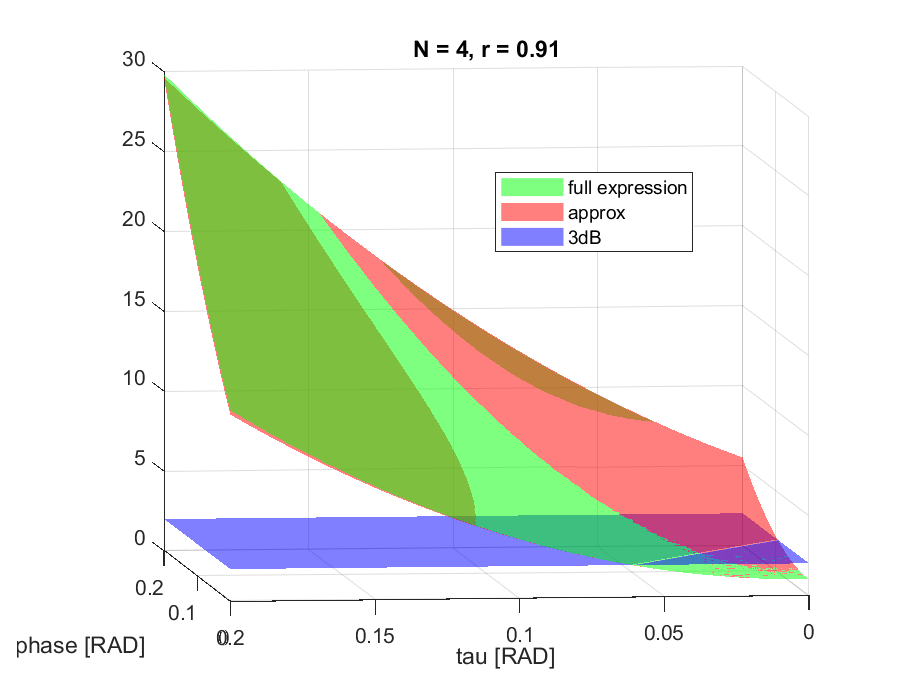
\includegraphics[width=0.9\linewidth]{./Media/spatial_IIR_MATLAB/beamwidth/BW_approx_validation.eps}
    \caption{Graphically comparing (\ref{eqn_arrayPerformance_beamwidth_fullEpxr}) and (\ref{eqn_arrayPerformance_beamwidth_approx}) for $N=4$ and $\rho=0.91$. The approximation seems to closely match the original expression.}
\end{figure}
Unlike the passive ULA case, it is evident from figure (\ref{fig_singleFreqFeedback_2ndTaylorNumericalValidation}) that the $4^{th}$ order terms are not needed for the evaluation of $\theta_{HPBW}$. In perfect phase alignment (i.e. $\Delta_{\tau}=0$), the u-space expression for the HPBW is $$u_{HPBW} =
\frac{
\left|1-\rho\right|
}{
\pi{d}
}
\lambda
\sqrt{\frac{
12
}{
\left(N-1\right)\left(\left(1+2r\right)N-4r+1\right)
}}.
$$
Comparing to the classic ULA beamwidth \cite{VanTrees2002DetectionIV}, thoroughly discussed in appendix \ref{appendix_theULABeamwidth}, we can express the improvement factor as
$$
\frac{
0.89\frac{\lambda}{ND}
}{
\theta_{HPBW,IIR}
}
=
\frac{0.89}{\left|1-\rho\right|}\sqrt{\frac{1+2r}{12}}
$$
\todo{TODO}
\textbf{Add graph of the improvement factor}
% \subsection{The pole-based design approach}
% In this approach, we look for setting the response "poles" which minimize the denominator, thus maximizing the overall response magnitude. To evaluate the beamwidth, we chose to allocate all of the system's poles in a single position such that 
% $
% 1-\vecnot{\beta}^{T}\vecnot{d}_{\theta}e^{-j\tau}
% =
% \left(e^{j\theta}-re^{j\theta_{s}}\right)^{N}
% $
% where $N$ is the number of array sensors and $r \in \left[0,1\right)$ enables us to avoid treatment of $\infty$-valued expressions. Next, we look for $\theta$ such that
% $
% \left|\frac{
% \frac
% {
% \vecnot{\alpha}^{T}\vecnot{d}_{\theta_{s}}
% }{
% \vecnot{\beta}^{T}\vecnot{d}_{\theta_{s}}
% }
% }{
% \frac
% {
% \vecnot{\alpha}^{T}\vecnot{d}_{\theta}
% }{
% \vecnot{\beta}^{T}\vecnot{d}_{\theta}
% }
% }\right|
% = \frac{1}{\sqrt{2}}
% $. Assuming that, like in classical IIR filter design theory, the numerator behaviour is significantly "slower" than the denominator's which results in $\vecnot{\alpha}^{T}\vecnot{d}_{\theta} 
% \approx
% \vecnot{\alpha}^{T}\vecnot{d}_{\theta_{s}}$ reults in
% \begin{align*}
%     \left|\frac{
%     \vecnot{\beta}^{T}\vecnot{d}_{\theta}
%     }{
%     \vecnot{\beta}^{T}\vecnot{d}_{\theta_{s}}
%     }\right|
%     &= \frac{1}{\sqrt{2}}
%     \\
%     \left|
%     \frac{
%     \left(e^{j\theta}-re^{j\theta}\right)^{N}
%     }{
%     \left(e^{j\theta}-re^{j\theta_{s}}\right)^{N}
%     }
%     \right|
%     &=
%     \left|
%     \frac{
%     \left(1-re^{j\left(\theta_{s}-\theta\right)}\right)
%     }{
%     \left(1-r\right)
%     }
%     \right|^{N}
%     \\
%     &=
%     \left|
%     \frac{
%     1+r^{2}-2r\cos{\left(\theta_{s}-\theta\right)}
%     }{
%     \left(1-r\right)^{2}
%     }
%     \right|^{\frac{N}{2}}
%     =
%     \left(\frac{1}{2}\right)^{\frac{1}{2}}
%     \\
%     \Rightarrow 
%     1+r^{2}-2r\cos{\left(\theta_{s}-\theta\right)}
%     &=
%     \left(1-r\right)^{2}2^{\frac{1}{N}}
%     \\
%     \cos{\left(\theta_{s}-\theta\right)}
%     &=
%     \frac{
%     1+r^{2}-\left(1-r\right)^{2}2^{\frac{1}{N}}
%     }{
%     2r
%     }
%     \\
%     \Rightarrow
%     \frac{\omega{D\left(cos(\theta_{g,s})-cos(\theta_{g,B})\right)}}{c}
%     &=
%     cos^{-1}
%     \left(
%     \frac{1+r^{2}-\left(1-r\right)^{2}2^{\frac{1}{N}}}{2r}
%     \right)
% \end{align*}.
% Therefore,
% \begin{equation}
%     \theta_{g,B} 
%     &= 
%     cos^{-1}
%     \left(
%     cos(\theta_{g,s})
%     -
%     \frac{c}{\omega{D}}
%     cos^{-1}
%     \left(
%     \frac{1+r^{2}-\left(1-r\right)^{2}2^{\frac{1}{N}}}{2r}
%     \right)
%     \right)
% \end{equation}
% Few observations can be derived from the $ \theta_{g,B} $:
% \begin{itemize}
%     \item $r\rightarrow{1}$ (i.e. setting the pole on the unit circle) causes $\theta_{g,B}\rightarrow\theta_{g,s}$ due to the $\infty$ valued response at $\theta_{g,s}$
%     \item The interval 
%     $
%     \left\{
%     \theta_{g,s}
%     \ \Bigg{|}\ 
%     cos(\theta_{g,s})
%     -
%     \frac{c}{\omega{D}}
%     cos^{-1}
%     \left(
%     \frac{1+r^{2}-\left(1-r\right)^{2}2^{\frac{1}{N}}}{2r}
%     \right)
%     <-1
%     \right\}
%     $, has no solution. In simulations, when evaluating such $\theta_{g,s}$ values, one can observe that the actual beampattern does not resemble the designed one due to the ULA geometric properties.
%     \item The number of sensors $N$ seems to have low impact on the beamwidth.
% \end{itemize}
\subsection*{Location of sidelobes and the rate of decrease}
Unlike the passive ULA case, it is clear from (\ref{eqn_arrPerformance_beamwidth_3dB}) that the positions of the feedback based beampattern sidelobes are affected both by the numerator and the denominator of $\Hr_{\dTheta}$. Considering the \coefSetName{} approach (i.e. single DOA enhancement), the denominator has only one single minima on the main lobe. Therefore, the sidelobes positions, same as the ULA case, are known \cite{VanTrees2002DetectionIV} to be 
\begin{equation}
    \label{eqn_CB_sidelobesLocations}
    \dTheta_{\coefSetName{},\text{sidelobes}} = \frac{\rBrace{2m+1}\pi}{N}\ \forall m\in\cBrace{1,2,\hdots}.
\end{equation}
Our initial interest is the first sidelobe (i.e. $m=1$), therefore we express the normalized beampattern at $\dTheta = \frac{3\pi}{N}$ (and setting $\dPhi=0$ for objective comparison). It can easily be verified that 
\begin{equation*}
    \Hr_{\frac{3\pi}{N}}
    =
    \frac{
    2\rBrace{1-r}^{2}
    }{
    \rBrace{N^{2}-2Nr}\rBrace{1-\cos{\rBrace{\frac{3\pi}{N}}}}+2r^{2}
    },
\end{equation*}
which for large $N$ values (as seen in Fig.~\ref{fig_firstSidelobeGain_CB}), can be well approximated by
\begin{equation*}
    \sqrt{\Hr_{\frac{3\pi}{N}}}
    \overset{N\gg1}{\approx}
    \frac{
    2\rBrace{1-r}
    }{
    3\pi
    }.
\end{equation*}
\begin{figure}[t!]
    \begin{center}
        \begin{overpic}[width=.75\linewidth, 
        %grid, 
        tics=10,trim=0 0 0 0]{./Media/spatial_IIR_MATLAB/arrayParameters/firstSidelobeGain_vs_N_various_r.eps}
            \put (6, 72){\footnotesize{$\Hr_{\frac{3\pi}{N}}{}$ - First sidelobe gain}}
            \put (20, 54) {\footnotesize{$r=0$ (i.e. no feedback)}}
            \put (20, 42) {\footnotesize{$r=0.3$}}
            \put (20, 33) {\footnotesize{$r=0.5$}}
            \put (20, 24) {\footnotesize{$r=0.7$}}
            \put (20, 14) {\footnotesize{$r=0.9$}}
            \put (-3, 50.5) {{$\frac{2\rBrace{1-0}}{3\pi}$}}
            \put (-3, 37.5) {{$\frac{2\rBrace{1-0.3}}{3\pi}$}}
            \put (-3, 28.5) {{$\frac{2\rBrace{1-0.5}}{3\pi}$}}
            \put (-3, 20) {{$\frac{2\rBrace{1-0.7}}{3\pi}$}}
            \put (-3, 12) {{$\frac{2\rBrace{1-0.9}}{3\pi}$}}
            \put (50, 2) {\footnotesize{$N$}}
        \end{overpic}
    \end{center}
    \caption{Plot of $\Hr_{\frac{3\pi}{N}}{}$ (i.e. the first sidelobe gain) vs. N for various $r$ values. The expected limit values (for large $N$) are presented as horizontal lines for each instance of $r$. Evidently, as expected, the gains tend to unite with the matching limits. $r=0$ is of special importance, being the reference for evaluation of the integrated feedback related improvement.}
    \label{fig_firstSidelobeGain_CB}
\end{figure}
It follows that, comparing to the known \cite{VanTrees2002DetectionIV} result of the passive ULA case (i.e. first sidelobe gain of $\frac{2}{3\pi}$), the first sidelobe gain improvement factor under the \coefSetName{} approach is
\begin{equation}
    \mu_{\text{first-sidelobe-gain,\coefSetName{}}} = \frac{1}{1-r}.
\end{equation}
Since the denominator magnitude, under the \coefSetName{} approach, is practically flat when not around the main lobe, the rate of sidelobes decay stays approximately the same as the numerators, which is similar to the known \cite{VanTrees2002DetectionIV} passive ULA sidelobe decay rate of $1/\rBrace{2m+1}$ (where $m$ is the sidelobe index).
\subsection*{Array directivity}
Another common measure for the array performance is the directivity \cite{VanTrees2002DetectionIV}, $\text{D}$. In the context of this work, considering the steer error scenario, it is defined as
\begin{equation*}
    \text{D}_{\coefSetName{}} = \frac{\Hr_{0}}{\frac{1}{2\pi}\int^{0}_{2\pi}\Hr_{\dTheta}\ d\dTheta},
\end{equation*}
measuring the ratio between the maximal array gain to the averaged gains in all directions. For uniformly weighted passive ULAs, assuming normalized beampattern, it is known \cite{VanTrees2002DetectionIV} that $D = N$.
\par Numerically sweeping various $\vBrace{N,r}$ sets, unveils that
\begin{equation}
    \text{D}_{\coefSetName{}} = \frac{r^{2}-\rBrace{N-1}r+N}{\rBrace{r-1}^{2}},
\end{equation}
matching the passive ULA result (i.e. $\evalat{D_{ULA}}{r=0}=N$), which leads to expressing the \coefSetName{} directivity improvement factor 
\begin{equation}
    \mu_{\text{D},\coefSetName{}}= \frac{r^{2}-\rBrace{N-1}r+N}{N\rBrace{r-1}^{2}}\overset{N\to\infty}{\to}\frac{1}{\rBrace{r-1}}.
\end{equation}
It is worth mentioning that for $\vBrace{r\to1,N\gg1}$ value sets, classic numerical approximations for the integral fail around $\dTheta\to0$ due to the the fact that both the numerator and the denominator tend to 0 (known to have a finite limit of 1 for $\dTheta=0$), forcing symbolic evaluation which was achieved using MATHEMATICA.
\section{Range Error Sensitivity}
\label{sec_sim}
In this section we investigate $\HrTPr$ for the general case, where also range misalignment phase term $\dPhi$ is possibly non zero. In Fig.~\ref{fig_hDUDTContour}, we plot $\abs{\HrTPr}$ in logarithmic scale, with respect to both steer and range misalignments.
Close inspection of the range error related beampattern behaviour sheds light to some important observations.
First, we notice that although setting $r\to1$ (i.e. close to perfect gain match), sharpens the beampattern's main lobe  (i.e. higher spatial selectivity), it also amplifies the range error ($\dPhi$) related sensitivity as the main lobe's support over the $\dPhi/\pi$ axis shrinks. 
Next, as evident from \eqref{eq_generalH}, the range error related sensitivity is $2\pi$-periodic with respect to $\dPhi$ (see Fig.~\ref{fig_hDUDTContour_mutliPeak}).
To establish our final observation, we first recall that
\[
\phi\triangleq\omega\tau_{pd}=\frac{2\pi R_{\text{rt}}}{\lambda},
\]
where $R_{\text{rt}}=2R$ is the round-trip distance between the array and the target of interest and denote
\[
\Delta R_{\text{rt}}\omegaB=\frac{\dPhi\lambda}{2\pi} 
\]
as the range estimation error.
Then, simulating different range estimation errors in Fig.~\ref{fig_rangError} shows that even minor range errors of $\Delta R_{\text{rt}}\sim0.1\lambda$ significantly distort the beampattern.
\begin{figure}[t!]
    \begin{center}
        \begin{overpic}[width=.95\linewidth, 
        % grid, 
        tics=10,
        % trim={<left> <lower> <right> <upper>}
        trim={0cm 0cm 1.5cm 0cm}
        ]{./Media/spatialIIR_amb_N3_all_r.eps}
            \put (91, 74) {\footnotesize{dB}}
            \put (-2, 22) {$\frac{\dPhi}{\pi}$}
            \put (5, 74) {\footnotesize{$r=0.4$}}
            \put (51, 74) {\footnotesize{$r=0.6$}}
            \put (5, 38) {\footnotesize{$r=0.7$}}
            \put (51, 38) {\footnotesize{$r=0.8$}}
            \put (19, 3) {\footnotesize{$\dTheta/\pi$}}
        \end{overpic}
    \end{center}
    \caption{Evaluation of $10\log_{10}\abs{\Hr_{\dTheta,\dPhi,r}}^2$, considering both steer ($\dTheta$) and range related ($\dPhi$) errors. Centered in each plot, is the 3dB main lobe (white color fill), exemplifying that as the gain mismatch $r$ is set closer to one, we observe an increase of the spatial selectivity (regarding  both $\dTheta$ and $\dPhi$).}
  \label{fig_hDUDTContour}
\end{figure}
\begin{figure}[t!]
    \begin{center}
        \begin{overpic}[width=0.6\linewidth, 
        % grid, 
        tics=10,
        % trim={<left> <lower> <right> <upper>}
        trim={0 0 0 0}
        ]{./Media/spatialIIR_amb_N3r04_multiPeak.eps}
            \put (83, 71) {\tiny{dB}}
            \put (42, -0.5) {\scriptsize{$\dTheta/\pi$}}
            \put (0, 37) {$\frac{\dPhi}{\pi}$}
        \end{overpic}
    \end{center}
    \caption{Evaluation of $10\log_{10}\abs{\Hr_{\dTheta,\dPhi,r=0.4}}^2$ for $-3\pi\leq\dPhi\leq 3\pi$. The response is $2\pi$ periodic.}
  \label{fig_hDUDTContour_mutliPeak}
\end{figure}
\begin{figure}[t!]
    \begin{center}
        \begin{overpic}[width=0.7\linewidth, 
        % grid, 
        tics=10,
        % trim={<left> <lower> <right> <upper>}
        trim={0 0 0 0}
        ]{./Media/rangeError_r06.eps}
            \put (-1, 74) {\footnotesize{$10\log_{10}\abs{\Hr_{\dTheta,\dPhi,r}}^2$}}
            \put (46, -1) {\footnotesize{$\dTheta/\pi$}}
            \put (0, 37) {\footnotesize{dB}}
            \put (92, 40) {\footnotesize{$\Delta R_{\text{rt}}=0.1\lambda$}}
            \put (92, 50) {\footnotesize{$\Delta R_{\text{rt}}=0.3\lambda$}}
            \put (92, 30) {\footnotesize{$\Delta R_{\text{rt}}=0$}}
        \end{overpic}
    \end{center}
    \caption{Evaluation of the array response for several values of range error $\Delta R_{\text{rt}}$ (where $r=0.4$). Even minor range errors significantly distort the beampattern.}
  \label{fig_rangError}
\end{figure}
\par At first glance, this sensitivity to range errors renders the system being too sensitive for any practical use, leading us to seek robust implementations, as demonstrated in Sec.~\ref{sec_app}. 

\section{Mitigating Range Error Sensitivity}
\label{sec_app}
As demonstrated in the previous section, the beampattern \eqref{eq_generalH} is very sensitive to range errors.
We now propose an architecture which obtains the desired beampattern $\Hr_{\dTheta,\dPhi\to0,r}$ even when in practice, the true range to the target is unknown (i.e. $\Delta R_{rt}$ is large). Moreover, we intend to show that the suggested architecture operates at moderately low signal to noise ratio (SNR).

\subsection*{Motivation}
Bearing in mind that the system's phase alignment sensitivity resides in \eqref{eq_generalH} via the  term $\exp\Brack{j\dPhi}=\exp\Brack{j\omega\Delta\tau_{pd}}$, and that the round-trip delay (i.e. $\tau_{pd}$) cannot be controlled, one may suggest to use lower frequencies. Unfortunately, transmission of such low frequencies is physically unfeasible. 
\par Another approach is to simultaneously use several frequencies in order to resolve the range error sensitivity. In the following, we show a possible algorithm which achieves this goal by transmitting with two frequencies $\omega_1$ and $\omega_2$.

\subsection*{Suggested processing scheme}
\begin{figure}[t!]
    \begin{center}
        \begin{overpic}[width=0.95\linewidth, 
        % grid, 
        tics=10,trim={0 0 0 0}]{./Media/SpatialIIR_APP.png}
            \put (12.5, 64){$\text{FB}_{\vAlpha_{1},\vBeta_{1}}$}
            \put (61, 64){$\text{FB}_{\vAlpha_{2},\vBeta_{2}}$}
            \put (4.5, 59){$y_{1}\rBrace{t}$}
            \put (54, 59){$y_{2}\rBrace{t}$}
            \put (12.9, 41.5){$\text{BPF}_{\omega_{1}}$}
            \put (61.65, 41.5){$\text{BPF}_{\omega_{2}}$}
            \put (6, 51.5){+}
            \put (55, 51.5){+}
            \put (16, 51.5){\footnotesize{$n_{1}\rBrace{t}$}}
            \put (64.75, 51.5){\footnotesize{$n_{2}\rBrace{t}$}}
            \put (24.5, 59){\footnotesize{$\text{Tx}_{1}\rBrace{t}$}}
            \put (73.5, 59){\footnotesize{$\text{Tx}_{2}\rBrace{t}$}}
            \put (36.25, 64){\scriptsize{$x_{1}\rBrace{t}$}}
            \put (43, 64){\scriptsize{$x_{2}\rBrace{t}$}}
            \put (18.25, 13){\footnotesize{Harmonic mean}}
            \put (32, 2){$y\rBrace{t}$}
            \put (54.75, 24){$\Sigma$}
            \put (21.75, 25){\footnotesize{$\mathcal{F}_{\omega_{1}}$}}
            \put (30.75, 25){\footnotesize{$\mathcal{F}_{\omega_{2}}$}}
        \end{overpic}
    \end{center}
    \caption{Dual-frequency beamformer, consisting of two independent FB blocks and nerrwoband bandpass filters. The blocks marked by $\mathcal{F}_{\omega_{i}}$ compute the Fourier coefficients in $\omega_{i}$ and their outputs feed the harmonic mean calculator which generates the DF beamformer's output.}
    \label{fig_app}
\end{figure}
In Fig.~\ref{fig_app}, we exemplify the use of two independently configured instances of the feedback beamformer (of Fig.~\ref{fig:Proposed_spatialIIR_ARCH}), where each instance is designed to treat only a specific frequency. 
\par For this, two independent FB blocks and 4 nerrow-band band-pass-filters ($\text{BPF}_{\omega_{i}}$ filters a nerrow band slice around $\omega_{i}$) are used to generate both the transmitted feedback signal ($\text{Tx}_{i}$) and the beamformers' outputs $y_{i}$. 
\par Also, $x_{i}(t) = e^{j\omega_{i}t}, \omega_{i} = 2\pi{f_{i}}$ with $i=1,2$ are two independent, narrow band, stimuli signals and $n_{i}$ are additive noise instances. 
\par Note that we do not increase the number of array elements, but merely double the beamformer processing part. 
\par For each single frequency FB block \eqref{eqn:GeneralFeedbackTransferFunction} the output is
\[
y_{i}(t)=H_{\vAlpha_{i},\vBeta_{i}}\rBrace{\omega_{i}}\exp{\rBrace{j\omega_{i}t}}\ \ {i\in\cBrace{1,2}},
\]
where $\vAlpha_{i},\vBeta_{i}$ are the coefficients of the $i$'th beamformer. 
\par We define $H_{\text{DF}}$ to be the \textit{dual frequency} beamformer, which is computed as the harmonic mean of $H_{\vAlpha_{i},\vBeta_{i}}(\omega_i)$ 
\begin{equation*}
    H_{\text{DF}} = \rBrace{H^{-1}_{\vAlpha_{1},\vBeta_{1}}\rBrace{\omega_{1}}+H^{-1}_{\vAlpha_{2},\vBeta_{2}}\rBrace{\omega_{2}}}^{-1}.
\end{equation*}
In practice, $H_{\text{DF}}$ can be estimated by evaluating $y_1(t)$ and $y_2(t)$ in the frequency domain, as also illustrated in Fig.~\ref{fig_app}.

By straight forward derivations, one may deduce that $\lBrace{H_{\text{DF}}}^{-1}$ is
% \begin{equation*}
%     \resizebox{1\linewidth}{!}{
%         \begin{split}
%             \lBrace{H_{\text{DF}}} =
%             \lBrace{
%             \frac
%             {
%             \vBetaT_{1}\vd_{1}\vBetaT_{2}\vd_{2}
%             }{
%             \vBetaT_{2}\vd_{2}\exp{\rBrace{-j\rBrace{\phi_{1}-\phi_{2}}}}+\vBetaT_{1}\vd_{1}
%             -\rBrace{\vBetaT_{1}\vd_{1}\vAlphaT_{2}\vd_{2}+\vBetaT_{2}\vd_{2}\vAlphaT_{1}\vd_{1}}\exp{\rBrace{-j\phi_{2}}}
%             }
%             }.
%         \end{split}
%     }
% \end{equation*}
\begin{equation*}
    \resizebox{1\linewidth}{!}{
        \begin{split}
            \lBrace{
            \frac
            {
            \vBetaT_{2}\vd_{2}\exp{\rBrace{j\rBrace{\phi_{1}-\phi_{2}}}}+\vBetaT_{1}\vd_{1}
            }{
            \vBetaT_{1}\vd_{1}\vBetaT_{2}\vd_{2}
            }
            -
            \frac
            {
            \rBrace{\vBetaT_{1}\vd_{1}\vAlphaT_{2}\vd_{2}+\vBetaT_{2}\vd_{2}\vAlphaT_{1}\vd_{1}}\exp{\rBrace{-j\phi_{2}}}
            }{
            \vBetaT_{1}\vd_{1}\vBetaT_{2}\vd_{2}
            }
            }.
        \end{split}
    }
\end{equation*}
Note that in the special case of choosing $\vAlpha_{1}~=~\vBeta_{1},\ \vAlpha_{2}~=~-~\vBeta_2{}$, the resultant beampattern simplifies to
\begin{equation}
    \label{eqn_twoFreqApproach_h}
    \abs{H_{\text{DF}}} = \lBrace{\frac{\vBetaT_{1}\vd_{1}}{1+\frac{\vBetaT_{1}\vd_{1}}{\vBetaT_{2}\vd_{2}}\exp{\rBrace{-j\rBrace{\phi_{1}-\phi_{2}}}}}}.
\end{equation}
\par In the general case, the gain of each element is frequency dependant, such that the steering vector $\vd$ of \eqref{eq:d}
may be expressed as 
\begin{equation*}
    \vd_{\theta_g}[n] = g_{n,\theta_{g}}(\omega)\exp{\rBrace{-j\omega\tau_{n,\theta_g}}},\;n=0,\ldots,N-1.
\end{equation*}
To simplify the exposition, we assume common gain across the array (i.e. $g_{\theta_{g}}(\omega)$ is not a function of the element index $n$) and suppress the DOA ($\theta_g$) dependency (which is the same at both frequencies) such that one may express the $i$'th frequency steering vector as
\begin{equation}\label{eq:new_d}
\vd_{i}^T=g(\omega_i)\sBrack{\exp{\rBrace{-j\omega_i\tau_{0}}},...,\exp{\rBrace{-j\omega_i\tau_{N-1}}}}.
\end{equation}
\par Note that the element-wise delay $\tau_n$ is arbitrary, hence we no longer restrict the discussion to linear arrays or any specific array manifold. Also, as $\tau_n$ represents the inter-element delay, we use $\tau_0=0$ (i.e. treating sensor $0$ as the reference sensor).
\par We further simplify the second beamformer's weights to 
\begin{equation}\label{eq_simpleBeta}
    \vAlpha_{2}=-\vBeta_{2}=\vBrace{\hat{g}^{-1}(\omega_2),0,\hdots,0}.
\end{equation}
Plugging \eqref{eq_simpleBeta} into \eqref{eqn_twoFreqApproach_h} gives rise to 
\begin{equation}
    H_{\text{DF}} = \lBrace{\frac{\vBetaT_{1}\vd_{1}}{1+
    \rBrace{\vBetaT_{1}\vd_{1}/r_{2}}\exp\rBrace{-j\rBrace{\phi_{1}-\phi_{2}}}
    }},
    \label{eq_H_DF_general}
\end{equation}
where $r_i=g(\omega_i)/\hat{g}(\omega_i)$ is the gain mismatch at $\omega_i$. 
\par Notice that  $H_{\text{DF}}$ is similar to the single frequency (SF) beampattern \eqref{eqn:GeneralFeedbackTransferFunction}, where the range related phase $\phi$ is replaced by $\phi_{1}-\phi_{2}=(\omega_1-\omega_2)\tau_{pd}$. Hence, by using sufficiently close frequencies, one may significantly mitigate the range mismatch distortion of the beampattern.
\par For example, consider a radio frequency carrier of $10\text{GHz}$ and typical range error of $\Delta{}R_{rt}=10_m$, which is $333\frac{1}{3}\lambda$ (assuming light speed of $c=3\cdot 10^{8}_{m/s}$). The single frequency beampattern distortion, being periodic in $\lambda$, will closely resembles the $0.3\lambda$ error plot presented in Fig.~\ref{fig_rangError}. 
\par Assume that we aim at maximal phase error of $\Delta \phi=0.01\pi_{rad}$. Hence, when using the \textit{dual frequency} architecture, the dictated frequency relation is
\begin{equation}\label{eq_DF_phErr}
\abs{(\omega_1-\omega_2)\frac{\Delta{}R_{rt}}{c}}<0.01\pi.
\end{equation}
or equivalently, for maximal range error of $10_m$, frequency separation of
\[
\abs{f_1-f_2}<0.005 c/\Delta{}R_{rt}=150_{KHz}
\]
is required. 

\subsection*{Dual frequency $\coefSetName$ simulation}
We now simulate \eqref{eq_H_DF_general} for the $\coefSetName$ approach assuming ULA. Using coefficients $\vBeta_{1}$ which will coherently sum the wave-front, while minimizing the magnitude of the denominator, we use
\begin{equation*}
    \vBeta_{1}=-\hat{\vd}^{\ast}\exp\rBrace{j\rBrace{\hat{\phi}_{1}-\hat{\phi}_{2}}}/\norm{\hat{\vd}}^2
\end{equation*}
where $\hat{\vd}$ is the estimated steering vector, as in \eqref{eq:d_hat}. With this choice, and similarly to \eqref{eq:SF_CB}, \eqref{eq_H_DF_general} becomes
\begin{equation}
    \label{eqn_H_DF_CB}
    \resizebox{.89\linewidth}{!}{
        \begin{split}
            H_{\text{DF,CB}} =
            \lBrace{\frac{r_{1}\D{\dTheta/2}{N}}{1-
            \kappa\D{\dTheta/2}{N}\exp\rBrace{-j\rBrace{\dPhi_{2}-\dPhi_{1}+(N-1)\dTheta/2}}}
            },
        \end{split}
    }
\end{equation}
where $\kappa\triangleq{}r_{1}/r_{2}$ is the gain mismatch ratio.
\par Note that for close frequencies such that $r_{1}\sim{}r_{2}$, $\kappa$ tends towards unity, thus significantly mitigating the gain mismatch effect even when both feedback beamformers are mismatched.
\par In Fig.~\ref{fig_dualfreq_rangeErrorHighSnr}, we simulate the beampattern (normalized to $0$dB peak gain) for the single and \textit{dual frequency} architectures, where frequency separation was configured to obtain range errors as in \eqref{eq_DF_phErr} (i.e. $f_1=10_{GHz},\;f_2=f_1+150_{KHz}$ to mitigate range errors up till $\Delta{}R_{rt}=10_m=333\frac{1}{3}\lambda$). 
\par We also plot (in blue circles) the perfectly aligned pattern, which is obtained when there are no range errors. 
\par As can be seen, the resultant beampattern of the \textit{dual frequency} beamformer practically achieves the ideal, range-error free case. 

In Fig.~\ref{fig_dualfreq_perfectAlignLowSnr}
we repeat the case of fractional range error of $\Delta{}R_{rt}=0.3\lambda$, while adding white Gaussian noise to the output of each feedback beamformer. Evidently, the dual-frequency beamformer (green diamonds) achieves close-to-ideal beampattern (blue circles), while the single-frequency beamformer (red squares) suffers severe distortions.
\begin{figure}[t!]
    \begin{center}
        \begin{overpic}[width=.7\linewidth, 
        % grid, 
        tics=10,trim=0 0 0 0]{./Media/fig_dualfreq_rangeErrorHighSnr.eps}
            \put (48, 43){\scriptsize{Ideal}}
            \put (48, 37.5){\scriptsize{SF}}
            \put (48, 32){\scriptsize{DF}}
            \put (2, 37.5){\footnotesize{dB}}
            \put (47,0){\footnotesize{$\dTheta/\pi$}}
            \put (92,58){\footnotesize{$\Delta{}R_{rt}=0.3\lambda$}}
        \end{overpic}
    \end{center}
    \caption{Simulating 3 element ULA with $r_1=0.6^{2},\; r_2=0.6$ (hence $\kappa=0.6$) for infinite SNR. The (fractional) range error is $\Delta{}R_{rt}=0.3\lambda$.
    The ideal response is obtained for $\Delta{}R_{rt}=0$ (blue dots), with the single frequency (SF) beamformer (red squares) and the  dual-frequency (DF) solution (green diamonds). 
    }
    \label{fig_dualfreq_rangeErrorHighSnr}
\end{figure}
\begin{figure}[t!]
    \begin{center}
        \begin{overpic}[width=0.9\linewidth, 
        % grid, 
        tics=10,
        % trim={<left> <lower> <right> <upper>}
        trim={1.75cm 0 1.75cm 0}
        ]{./Media/fig_dualfreq_rangeErrorLowSnr.eps}
            \put (42.25, 17.5){\scriptsize{Ideal}}
            \put (42.25, 14.5){\scriptsize{SF}}
            \put (42.25, 11.5){\scriptsize{DF}}
            \put (-1, 26.5){\footnotesize{dB}}
            \put (22, 0){\footnotesize{$\dTheta/\pi$}}
            \put (19,17){\scriptsize{$\text{SNR}=6_{dB}$}}
            \put (71.5,17){\scriptsize{$\text{SNR}=0_{dB}$}}
        \end{overpic}
    \end{center}
    \caption{Directional response of the 3 element ULA, as in Fig.~\ref{fig_dualfreq_rangeErrorHighSnr}, simulated for the noisy scenario. The additive noises $n_1(t)$ and $n_2(t)$ (see Fig.~\ref{fig_app}), are set to obtain SNR of $6_{dB}$ (left plot) and $0_{dB}$ (right plot).}
    \label{fig_dualfreq_perfectAlignLowSnr}
\end{figure}
\section{Conclusions}
\label{sec_conclusions}
Integrating feedback into standard beamformers proved to achieve a spatial domain equivalent of the temporal IIR.
It seems that a simple generalization of the DS beamformer maximizes (locally) the system's residing spatial information, thus enabling high localization accuracy.
The feedback based architecture performance evaluation predicts an almost infinite improvement in all criteria, when considering perfect knowledge of the target's range and the channel attenuation.
It turns out that a single frequency waveform based FB is impractical, being too sensitive to even mild target range estimation errors.
Fortunately, using two frequency waveform and applying simple frequency domain manipulations to the output and feedback signals, were found to serve as a low frequency (hence low sensitivity) equivalent of the single frequency scheme.
Also, the dual frequency scheme proved to be of low noise sensitivity, featuring high performance even in relatively low SNR scenarios.
\par Future study of the FB concept may be applied to other array processing applications other than localization, inspect other interesting choices of coefficients rather than the DS generalization, suggest other waveforms and associated processing schemes, extend the results to dynamic/multiple targets, consider sensors with general radiation patterns etc.
Also, one may consider generalizing the suggested architecture to multiple input multiple output (MIMO) systems, enabling a steered/focused (rather than omni-directional) feedback transmission.
\appendices
\section{FIM calculation}
\label{apdx_clacFim}
Following \eqref{eq_beamPatternFreqDomain_FIM}, we elaborate the steps leading to \eqref{eqn_FIMelements}. First, we express the parial derivatives of $\F{y}$ with respect to $\vEta$, resulting in
\begin{equation*}
    \resizebox{.9\linewidth}{!}{
        \begin{split}
            \frac{\partial{\F{y}}}{\partial{\thetaD}} &= 
            \frac{
            \vBetaT{}A\omegaB\vd\ePhi{-}\rBrace{1-\aTd\ePhi{-}}+\bTd\vAlphaT{}A\omegaB\vd\ePhi{-2}
            }{
            \rBrace{1-\aTd\ePhi{-}}^{2}
            }
            \\&=
            \frac{
            \vBetaT{}A\omegaB\vd\ePhi{-}-\vBetaT{}\rBrace{A\omegaB\vd\vdT-\vd\vdT{}A\omegaB}\vAlpha\ePhi{-2}
            }{
            \rBrace{1-\aTd\ePhi{-}}^{2}
            }
            \\&=
            \frac{
            \vBetaT{}A\omegaB\vd\ePhi{-}-\vBetaT{}B\omegaB\vAlpha\ePhi{-2}
            }{
            \rBrace{1-\aTd\ePhi{-}}^{2}
            }
        \end{split}
    }
\end{equation*}
and
\begin{equation*}
    \resizebox{.9\linewidth}{!}{
        \begin{split}
            \frac{\partial{\F{y}}}{\partial{\phi}} &= 
            \frac{
            -j\bTd\ePhi{-}\rBrace{1-\aTd\ePhi{-}}-j\bTd\aTd\ePhi{-2}
            }{
            \rBrace{1-\aTd\ePhi{-}}^{2}
            }
            \\&=
            \frac{
            -j\bTd\ePhi{-}
            }{
            \rBrace{1-\aTd\ePhi{-}}^{2}
            }
        \end{split}
    }
\end{equation*}
such that
\begin{equation*}
    \resizebox{.9\linewidth}{!}{
        \begin{split}
            J_{\thetaD\thetaD} &= \Re\cBrace{\frac{1}{2\pi\sigma^{2}}\int_{-\omega_{s}/2}^{\omega_{s}/2}\lBrace{\frac{\partial{\F{y}\omegaB}}{\partial{\thetaD}}}^{2}d\omega}
            \\&=
            \frac{1}{2\pi\sigma^{2}}\int_{-\omega_{s}/2}^{\omega_{s}/2}{\frac{
            \lBrace{\vBetaT{}A\omegaB\vd-\vBetaT{}B\omegaB\vAlpha\ePhi{-}}^{2}
            }{
            \lBrace{1-\aTd\ePhi{-}}^{4}
            }\lBrace{\F{x}\omegaB}^{2}d\omega},
            \\
            J_{\phi\phi} &= \Re\cBrace{\frac{1}{2\pi\sigma^{2}}\int_{-\omega_{s}/2}^{\omega_{s}/2}\lBrace{\frac{\partial{\F{y}\omegaB}}{\partial{\phi}}}^{2}d\omega}
            \\&=
            \frac{1}{2\pi\sigma^{2}}\int_{-\omega_{s}/2}^{\omega_{s}/2}{\frac{
            \lBrace{\bTd}^{2}
            }{
            \lBrace{1-\aTd\ePhi{-}}^{4}
            }\lBrace{\F{x}\omegaB}^{2}d\omega}
        \end{split}
    }
\end{equation*}
and the cross terms are
\begin{equation*}
    \resizebox{.9\linewidth}{!}{
        \begin{split}
            &J_{\thetaD\phi} = J_{\phi\thetaD}^{\ast} = 
            \\&= \Re\cBrace{\frac{1}{2\pi\sigma^{2}}\int_{-\omega_{s}/2}^{\omega_{s}/2}
            \rBrace{\frac{\partial{\F{y}\omegaB}}{\partial{\phi}}}^{\ast}
            \frac{\partial{\F{y}\omegaB}}{\partial{\thetaD}}d\omega}
            \\&=
            \Re\cBrace{\frac{1}{2\pi\sigma^{2}}\int_{-\omega_{s}/2}^{\omega_{s}/2}{\frac{
            j\vBetaT{}\rBrace{A\omegaB\vd-B\omegaB\vAlpha\ePhi{-}}\vdH\vBetaC
            }{
            \lBrace{1-\aTd\ePhi{-}}^{4}
            }\lBrace{\F{x}\omegaB}^{2}d\omega}}.
        \end{split}
    }
\end{equation*}
Setting the coefficients as $$\vAlpha,\vBeta\propto\vd^{\ast}$$ causes the $\vBetaT{}B\omegaB\vAlpha$~term to vanish. Assuming real input and real gain terms $g_n$ within the steering vector, the function
\[
\frac{\lBrace{\F{x}\omegaB}^{2}}{\lBrace{1-\aTd\ePhi{-}}^{4}}
\]
is even with respect to $\omega$, and $$j\vBetaT{}A\omegaB\vd\vdH\vBetaC\propto A\omegaB\vd\norm{\vd}^2$$ is odd. Hence the cross terms vanish.

\section{Half power beamwidth}
\label{apdx_HPBW}
We now equate the squared norm of \eqref{eq_Hdphi0} to $0.5$ and compute the value of $N\dTheta/2$ for large $N$. Denoting $\gamma\triangleq\dTheta/2$,
\begin{equation*}
    \resizebox{1\linewidth}{!}{
        \begin{split}
            \abs{\Hr_{\dTheta,\dPhi=0,r}\rBrace{\omega}}^{2}&=
             \frac{\rBrace{1-r}^{2}\Dp{\gamma,N}{2}}{\abs{\exp\rBrace{j(N-1)\gamma}-r\D{\gamma}{N}}^{2}}
             \\&
             \overset{N\gg1}{\approx}\frac{\rBrace{1-r}^{2}\Dp{\gamma,N}{2}}{1-2r\cos{\rBrace{N\gamma}}\D{\gamma}{N}+r^{2}\Dp{\gamma,N}{2}}\overset{!}{=}\frac{1}{2},
        \end{split}
    }
\end{equation*}
which leads to 
\begin{equation*}
    % \resizebox{1\linewidth}{!}{
        \begin{split}
            \rBrace{r^{2}-4r+2}\Dp{\gamma,N}{2}+2r\cos{\rBrace{N\gamma}}\D{\gamma}{N}-1 = 0.
        \end{split}
    % }
\end{equation*}
Since for large $N$, the main lobe width goes to zero, we approximating $\sin(\gamma)$ with $\gamma$. Also defining $x\triangleq{}N\gamma=N\dTheta/2$ we obtain \eqref{eq_HPBW}.

\ifCLASSOPTIONcaptionsoff
  \newpage
\fi
\bibliographystyle{IEEEtran}
\bibliography{./Modules/Mendeley,./Modules/LocalBib}% ./Modules/LocalBib}
\begin{IEEEbiography}[{\includegraphics[width=1in,height=1.25in,clip,keepaspectratio]{./Media/addPhotoHere.PNG}}]{Israel Cohen}
(M’01–SM’03–F’15) He received the B.Sc. (Summa Cum Laude), M.Sc., and Ph.D. degrees in electrical engineering from the Technion – Israel Institute of Technology, Haifa, Israel, in 1990, 1993, and 1998, respectively.
He is currently a Professor of electrical engineering with the Technion – Israel Institute of Technology.
From 1990 to 1998, he was a Research Scientist with RAFAEL Research Laboratories, Israel Ministry of Defense, Haifa. 
From 1998 to 2001, he was a Postdoctoral Research Associate with the Computer Science Department, Yale University, New Haven, CT, USA. In 2001, he joined the Electrical Engineering Department, Technion – Israel Institute of Technology.
He is a coeditor of the Multichannel Speech Processing Section of the Springer Handbook of Speech Processing (Springer, 2008), and a coauthor of Fundamentals of Signal Enhancement and Array Signal Processing (Wiley-IEEE Press, 2017). 
His research interests include array processing, statistical signal processing, analysis and modeling of acoustic signals, speech enhancement, noise estimation, microphone arrays, source localization, blind source separation, system identification, and adaptive filtering.
Dr. Cohen was awarded the Norman Seiden Prize for Academic Excellence (2017), the SPS Signal Processing Letters Best Paper Award (2014), the Alexander Goldberg Prize for Excellence in Research (2010), and the Muriel and David Jacknow Award for Excellence in Teaching (2009). 
He is currently an Associate Member of the IEEE Audio and Acoustic Signal Processing Technical Committee. 
He was an Associate Editor for the IEEE TRANSACTIONS ON AUDIO, SPEECH, AND LANGUAGE PROCESSING and the IEEE SIGNAL PROCESSING LETTERS, and as Member of the IEEE Audio and Acoustic Signal Processing
Technical Committee and the IEEE Speech and Language Processing Technical Committee.
\end{IEEEbiography}
\begin{IEEEbiography}[{\includegraphics[width=1in,height=1.25in,clip,keepaspectratio]{./Media/addPhotoHere.PNG}}]{Tsvi G. Dvorkind}
Tsvi G. Dvorkind received the B.Sc. degree (summa cum laude) in computer engineering in 2000, the M.Sc. degree (summa cum laude) in electrical engineering in 2003, and the Ph.D. degree in electrical engineering in 2007, all from the Technion—Israel Institute of Technology, Haifa, Israel.
From 1998 to 2000 he worked at the Electro-Optics Research & Development Company at the Technion, and during 2000–2001 at the Jigami Corporation.
He is now with the Rafael Company, Haifa, Israel.
His research interests include speech enhancement and acoustical localization, general parameter estimation problems, and sampling theory.
\end{IEEEbiography}
\begin{IEEEbiography}{Itay Yehezkel Karo}
Biography text here.
\end{IEEEbiography}
\end{document}


